\section{Specific Requirement}

\subsection{External Interface Requirements}

\subsubsection{User Interfaces}

\subsubsection{Hardware Interfaces}

\subsubsection{Software Interfaces}

\subsubsection{Communication Interfaces}

\subsection{Functional Requirements}

    \subsubsection{Sequence Diagrams}
    
    \begin{figure}[h]
        \centering
        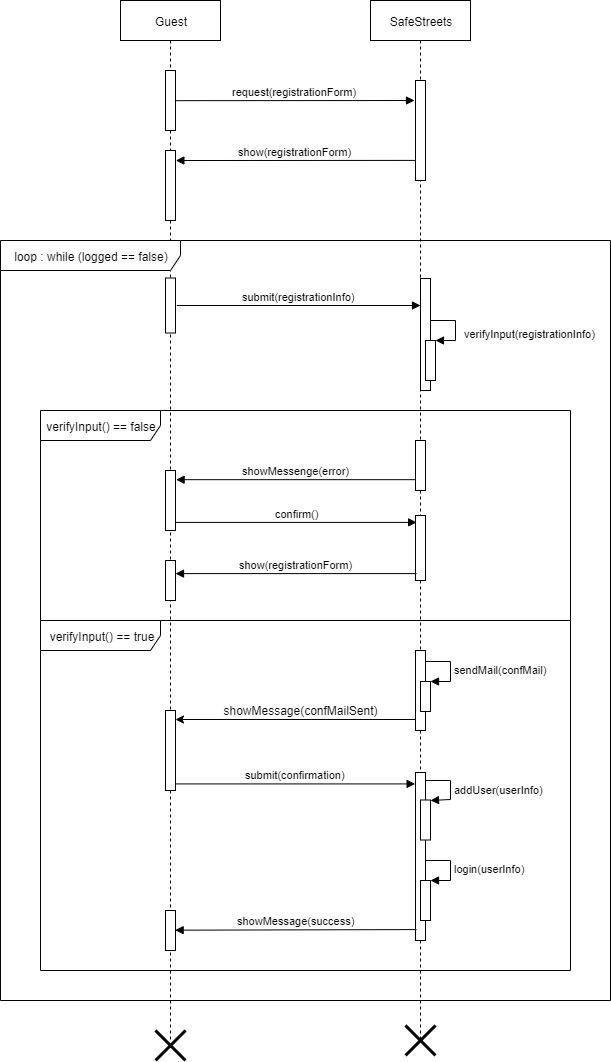
\includegraphics[scale=0.5]{SeqDiag_registration.png}
        \caption{Sequence Diagram of the registration of a User}
    \end{figure}
    
    \begin{figure}[h]
        \centering
        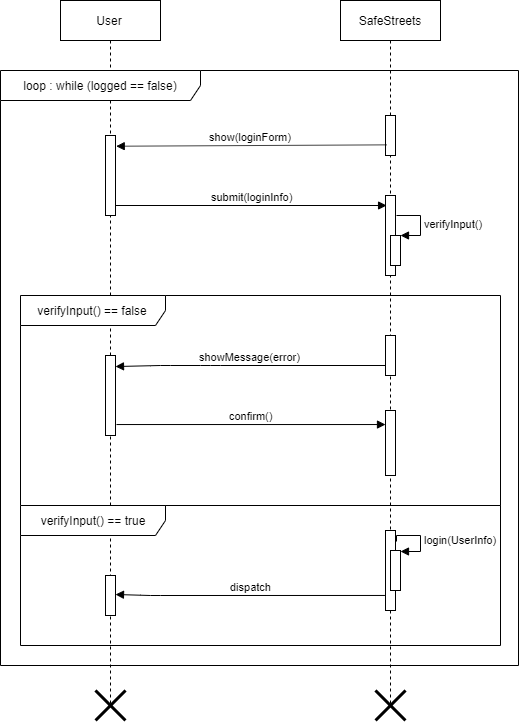
\includegraphics[scale=0.5]{SeqDiag_login.png}
        \caption{Sequence Diagram of the login of a User or of an Authority}
    \end{figure}
    
    \begin{figure}[h]
        \centering
        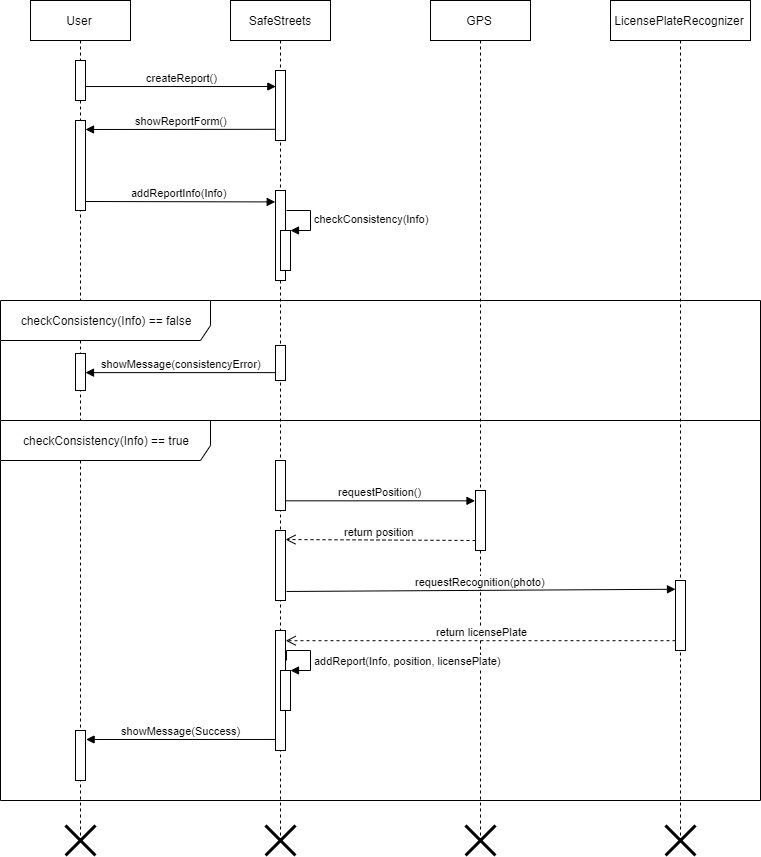
\includegraphics[scale=0.5]{SeqDiag_addReport.png}
        \caption{Sequence Diagram of the insertion of a Report by a User}
    \end{figure}
    
    \begin{figure}[h]
        \centering
        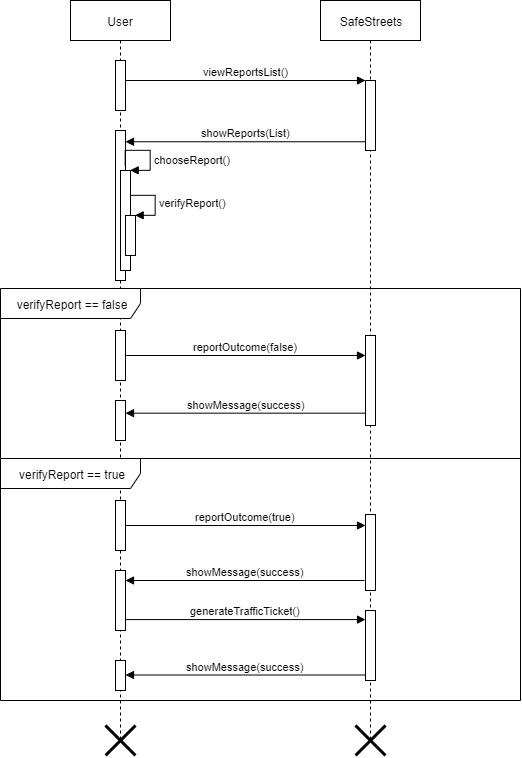
\includegraphics[scale=0.5]{SeqDiag_generateTrafficTicket.png}
        \caption{Sequence Diagram of the checking of a Report and, eventually, the generation of the corresponding Traffic Ticket}
    \end{figure}
    
    \begin{figure}[h]
        \centering
        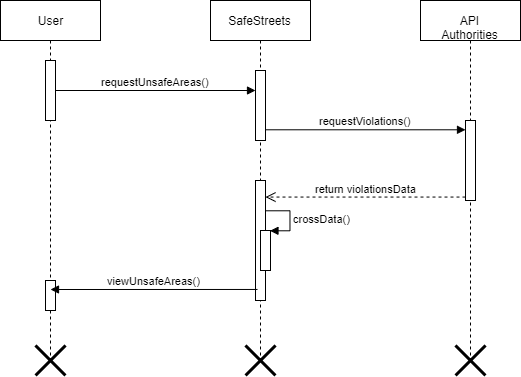
\includegraphics[scale=0.5]{SeqDiag_unsafeAreas.png}
        \caption{Sequence Diagram of the request to know which are the unsafe areas}
   \end{figure}

\subsection{Performance Requirements}

\subsection{Design
Constraints}

\subsubsection{Standards compliance}

\subsubsection{Hardware
limitations}

\subsubsection{Any other constraint}

\subsection{Software System Attributes}

\subsubsection{Reliability}

\subsubsection{Availability}

\subsubsection{Security}

\subsubsection{Maintainability}

\subsubsection{Portability}